\documentclass{beamer}

% Use metropolis theme
\usepackage[progressbar=foot]{theme/beamerthememetropolis}
\usepackage{minted}

\title{Intro to Lazy Evaluation}

\date{\today}
\author{Joe Jevnik}
\institute{PyCon 2017}

\begin{document}
\maketitle

\section{How do we execute programs?}

\begin{frame}[fragile]{How does Python Evaluate Expressions?}
  \begin{itemize}
  \item[]<1-> \begin{minted}{python}
>>> def f(a, b):
...     """An arbitrary binary function.
...     """
...     print(f'calling f with a={a}, b={b}')
...     return a + b
    \end{minted}
  \item[]<2-> \begin{minted}{python}
>>> a = f(1, 2)
calling f with a=1, b=2
    \end{minted}
  \item[]<3-> \begin{minted}{python}
>>> a
3
    \end{minted}
  \item[]<4-> \begin{minted}{python}
>>> b = f(a, 4)
calling f with a=3, b=4
    \end{minted}
  \item[]<5-> \begin{minted}{python}
>>> b
7
    \end{minted}
  \end{itemize}
\end{frame}

\section{Evaluation Models}

\begin{frame}{Eager Evaluation}
  \begin{definition}[Eager Evaluation]
    \begin{itemize}
    \item[]<2-> Evaluate expressions as they appear in source.
    \item[]<3-> Evaluate expressions inner-most first.
    \item[]<4-> Expressions immediately evaluate to a concrete value.
    \end{itemize}
  \end{definition}
\end{frame}

\begin{frame}{Eager Evaluation}
  \begin{block}{Eager Evaluation is a choice}
    \begin{itemize}
    \item[]<2-> Easy to reason about behavior.
    \item[]<3-> Easy to reason about performance.
    \item[]<4-> Easy to debug.
    \end{itemize}
  \end{block}
\end{frame}

\section{Lazy Evaluation}

\begin{frame}{Lazy Evaluation}
  \begin{definition}[Lazy Evaluation]
    \begin{itemize}
    \item[]<2-> Evaluate expressions as their result is needed.
    \item[]<3-> Evaluate expressions outer-most first.
    \item[]<4-> Expressions must be \textbf{pure}.
    \item[]<5-> Expressions produce \textbf{thunks}.
    \end{itemize}
  \end{definition}
\end{frame}

\begin{frame}{Lazy Evaluation}
  \begin{definition}[Thunk]
    \begin{itemize}
    \item[]<2-> Represents a computation which may or may not be evaluated.
    \item[]<3-> Term of art.
    \item[]<4-> Also known as a \textbf{closure}.
    \end{itemize}
  \end{definition}
\end{frame}

\begin{frame}{Lazy Evaluation}
  \begin{block}{Tools from Python}
    \begin{itemize}
      \item[]<2-> Functions and lambdas
      \item[]<3-> Iterators and generators
    \end{itemize}
  \end{block}
\end{frame}

\begin{frame}[fragile]{Lazy Evaluation}
  \begin{itemize}
  \item[]<1-> \begin{minted}{python}
>>> a = lambda: f(1, 2)
    \end{minted}
  \item[]<2-> \begin{minted}{python}
>>> a
<function <lambda> at 0x7fc7f5a6ef28>
    \end{minted}
  \item[]<3-> \begin{minted}{python}
>>> b = lambda: f(a(), 4)
    \end{minted}
  \item[]<4-> \begin{minted}{python}
>>> b
<function <lambda> at 0x7fc7f56d0b70>
    \end{minted}
  \item[]<5-> \begin{minted}{python}
>>> b()
calling f with a=1, b=2
calling f with a=3, b=4
7
    \end{minted}
  \end{itemize}
\end{frame}

\section{Expressions as Trees}

\begin{frame}{Expressions as Trees}
  \begin{center}
    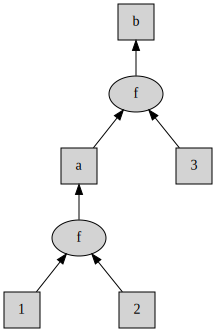
\includegraphics[height=0.75\textheight]{graphs/tree-full.png}
  \end{center}
\end{frame}

\begin{frame}{Expressions as Trees}
  \begin{center}
    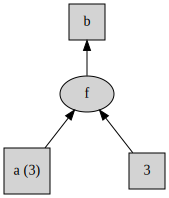
\includegraphics[height=0.65\textheight]{graphs/tree-computed.png}
  \end{center}
\end{frame}

\begin{frame}[fragile]{Expressions as Trees}
  \begin{itemize}
    \item[]<1-> \begin{minted}{python}
>>> a = 1
>>> b = 2
>>> sub_expression = f(a, b)
    \end{minted}
  \item[]<2-> \begin{minted}{python}
>>> value = lambda: f(
...    sub_expression(),
...    sub_expression(),
... )
    \end{minted}
  \item[]<3-> \begin{minted}{python}
>>> value()
calling f with a=1, b=2
calling f with a=1, b=2
falling f with a=3, b=3
6
    \end{minted}
  \end{itemize}
\end{frame}

\begin{frame}{Expressions as Trees}
  \begin{center}
    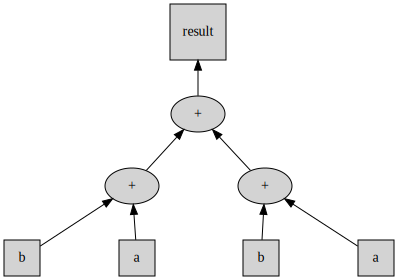
\includegraphics[height=0.75\textheight]{graphs/redundant-tree.png}
  \end{center}
\end{frame}

\begin{frame}{Expressions as Trees}
  \begin{center}
    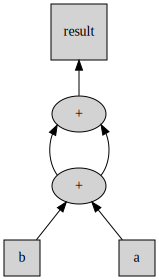
\includegraphics[height=0.75\textheight]{graphs/dag.png}
  \end{center}
\end{frame}

\section{Thunks}

\begin{frame}[fragile]{Na\"ive Thunks}
  \begin{block}{Na\"ive Thunks}
    \begin{itemize}
    \item[]<2-> \begin{minted}{python}
lambda: f(a, b)
      \end{minted}
    \item[]<3-> Simple
    \item[]<4-> Slow
    \item[]<5-> Does not take advantage of function purity
    \end{itemize}
  \end{block}
\end{frame}

\begin{frame}{Memoization}
  \begin{definition}[Memoize]
    \begin{itemize}
    \item[]<2-> Remembering the result of a computation.
    \item[]<3-> Repeated access to an expression can return instantly.
    \item[]<4-> Requires pure functions.
    \end{itemize}
  \end{definition}
\end{frame}

\begin{frame}[fragile]{Evaluating Thunks}
  \begin{minted}{python}
class Thunk(metaclass=ABCMeta):
    @abstractmethod
    def __call__(self):
        raise NotImplementedError()

def evaluate(expr):
    while isinstance(expr, Thunk):
        expr = expr()
    return expr
  \end{minted}
\end{frame}

\begin{frame}[fragile]{Cell Thunks}
  \begin{minted}{python}
class CellThunk(Thunk):
    not_evaluated = object()

    def __init__(self, code, *args, **kwargs):
        self.code = code
        self.args = args
        self.kwargs = kwargs
        self.value = self.not_evaluated
  \end{minted}
\end{frame}

\begin{frame}[fragile]{Cell Thunks}
  \begin{minted}{python}
def __call__(self):
    if self.value is self.not_evaluated:
        self.value = self.code(
            *(evaluate(arg) for arg in self.args),
            **{
                key: evaluate(value)
                for key, value in self.kwargs.items()
            },
        )
        del self.code
        del self.args
        del self.kwargs

    return self.value
  \end{minted}
\end{frame}

\begin{frame}[fragile]{Cell Thunks}
  \begin{itemize}
  \item[]<1-> \begin{minted}{python}
>>> a = CellThunk(1)
>>> b = CellThunk(2)
    \end{minted}
  \item[]<2-> \begin{minted}{python}
>>> sub_expression = CellThunk(f, a, b)
    \end{minted}
  \item[]<3-> \begin{minted}{python}
>>> value = CellThunk(
...     f,
...     sub_expression,
...     sub_expression,
)
    \end{minted}
  \item[]<4-> \begin{minted}{python}
>>> value()
calling f with a=1, b=2
calling f with a=3, b=3
6
    \end{minted}
  \end{itemize}
\end{frame}

\begin{frame}[fragile]{Self Updating Thunks}
  \begin{minted}{python}
class SelfUpdatingThunk:
    @staticmethod
    def indirection_code(value):
        return value
  \end{minted}
\end{frame}

\begin{frame}[fragile]{Self Updating Thunks}
  \begin{minted}{python}
    def __init__(self, code, *args, **kwargs):
        def update_frame(*args, **kwargs):
            value = code(*args, **kwargs)

            self.code = self.indirection_code
            self.args = (value,)
            self.kwargs = {}

            return value

        self.code = update_frame
        self.args = args
        self.kwargs = kwargs
  \end{minted}
\end{frame}

\begin{frame}[fragile]{Self Updating Thunks}
  \begin{minted}{python}
    def __call__(self):
        return self.code(
            *(evaluate(arg) for arg in self.args),
            **{
                key: evaluate(value)
                for key, value in self.kwargs.items()
            },
        )
  \end{minted}
\end{frame}

\begin{frame}[fragile]{Self Updating Thunks}
  \begin{itemize}
  \item[]<1-> \begin{minted}{python}
>>> a = SelfUpdatingThunk(1)
>>> b = SelfUpdatingThunk(2)
    \end{minted}
  \item[]<2-> \begin{minted}{python}
>>> sub_expression = SelfUpdatingThunk(f, a, b)
    \end{minted}
  \item[]<3-> \begin{minted}{python}
>>> value = SelfUpdatingThunk(
...     f,
...     sub_expression,
...     sub_expression,
)
    \end{minted}
  \item[]<4-> \begin{minted}{python}
>>> value()
calling f with a=1, b=2
calling f with a=3, b=3
6
    \end{minted}
  \end{itemize}
\end{frame}

\begin{frame}{Thunk Comparison}
  \begin{columns}[c]

    \column{0.33\textwidth}
    \begin{block}{Na\"ive}
      \begin{enumerate}
      \item Simple
      \item No state
      \end{enumerate}
    \end{block}

    \column{0.33\textwidth}
    \begin{block}{Cell Model}
      \begin{enumerate}
      \item Moderately complex
      \item Simple state
      \end{enumerate}
    \end{block}

    \column{0.33\textwidth}
    \begin{block}{Self Updating}
      \begin{enumerate}
      \item Most complex
      \item Complex state
      \end{enumerate}
    \end{block}
  \end{columns}
\end{frame}

\section{More Memoization}

\begin{frame}[fragile]{Reducing the Graph}
  \begin{itemize}
  \item[]<1-> \begin{minted}{python}
>>> a = CellThunk(1)
>>> b = CellThunk(2)
    \end{minted}
  \item[]<2-> \begin{minted}{python}
>>> sub_expression_1 = CellThunk(f, a, b)
    \end{minted}
  \item[]<3-> \begin{minted}{python}
>>> sub_expression_2 = CellThunk(f, a, b)
    \end{minted}
  \item[]<4-> \begin{minted}{python}
>>> result = CellThunk(
      f,
      sub_expression_1,
      sub_expression_2,
)
    \end{minted}
  \item[]<5-> \begin{minted}{python}
>>> result()
calling f with a=1, b=2
calling f with a=1, b=2
calling f with a=3, b=3
6
    \end{minted}
  \end{itemize}
\end{frame}

\begin{frame}{Reducing the Graph}
  \begin{center}
    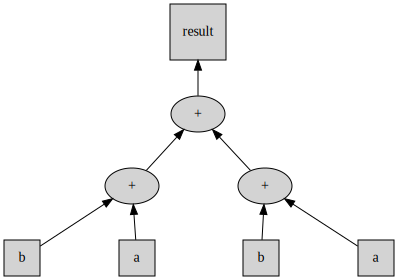
\includegraphics[height=0.75\textheight]{graphs/redundant-tree.png}
   \end{center}
\end{frame}

\begin{frame}[fragile]{Reducing the Graph}
  \begin{minted}{python}
thunk_cache = {}

def memoized_thunk(code, *args, **kwargs):
    key = (code, args, frozenset(kwargs.items()))
    try:
        thunk = thunk_cache[key]
    except KeyError:
        thunk = CellThunk(code, *args, **kwargs)
        thunk_cache[key] = thunk

    return thunk
  \end{minted}
\end{frame}

\begin{frame}[fragile]{Reducing the Graph}
  \begin{itemize}
  \item[]<1-> \begin{minted}{python}
>>> a = memoized_thunk(1)
>>> b = memoized_thunk(2)
    \end{minted}
  \item[]<2-> \begin{minted}{python}
>>> sub_expression_1 = memoized_thunk(f, a, b)
    \end{minted}
  \item[]<3-> \begin{minted}{python}
>>> sub_expression_2 = memoized_thunk(f, a, b)
    \end{minted}
  \item[]<4-> \begin{minted}{python}
>>> result = memoized_thunk(
      f,
      sub_expression_1,
      sub_expression_2,
)
    \end{minted}
  \item[]<5-> \begin{minted}{python}
>>> result()
calling f with a=1, b=2
calling f with a=3, b=3
6
    \end{minted}
  \end{itemize}
\end{frame}

\begin{frame}[fragile]{Reducing the Graph}
  \begin{minted}{python}
>>> sub_expression_1 is sub_expression_2
True
  \end{minted}
\end{frame}

\begin{frame}{Optimizations}
  \begin{center}
    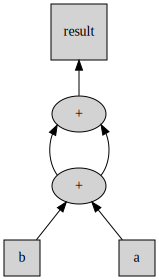
\includegraphics[height=0.75\textheight]{graphs/dag.png}
  \end{center}
\end{frame}

\section{``Real'' Example}

\begin{frame}[fragile]{Example}
  \begin{minted}{python}
def fib(n):
    if n <= 2:
        return 1

    return fib(n - 1) + fib(n - 2)
  \end{minted}
\end{frame}

\begin{frame}{Example}
  \begin{align*}
    fib(5) & : 850 ns \\
    fib(10) & :10.4 \mu s \\
    fib(15) & : 116 \mu s \\
    fib(20) & : 1.28 ms \\
    ... & : ... \\
    fib(100) & : ...
  \end{align*}
\end{frame}

\begin{frame}{Example}
  \begin{center}
    \includegraphics[height=0.75\textheight]{graphs/fib-bad.png}
  \end{center}
\end{frame}

\begin{frame}[fragile]{Example}
  \begin{minted}{python}
import operator as op


def lazy_fib(n):
    if n <= 2:
        return 1

    return memoized_thunk(
        op.add,
        memoized_thunk(fib, n - 1),
        memoized_thunk(fib, n - 2),
    )
  \end{minted}
\end{frame}

\begin{frame}{Example}
  \begin{align*}
    lazy\_fib(5)() & : 3.96 \mu s \\
    lazy\_fib(10)() & : 3.96 \mu s \\
    lazy\_fib(15)() & : 4.03 \mu s \\
    lazy\_fib(20)() & : 4.07 \mu s \\
    ... & : ... \\
    lazy\_fib(100)() & : 4.02 \mu s
  \end{align*}
\end{frame}

\begin{frame}{Example}
  \begin{center}
    \includegraphics[height=0.75\textheight]{graphs/fib-good.png}
  \end{center}
\end{frame}

\begin{frame}{Further Work}
  \begin{itemize}
  \item[]<2-> lazy\_python
    \begin{itemize}
    \item[] Implementation of Cell Model thunks for Python
    \end{itemize}
  \item[]<3-> daisy
    \begin{itemize}
    \item[] Uses lazy\_python to execute Python programs in parallel with Dask.
    \end{itemize}
  \item[]<4-> Poster Session
  \end{itemize}
\end{frame}

\begin{frame}{Thank You!}
  \begin{itemize}
  \item github.com/llllllllll/lazy-talk (ten lowercase ``L'' characters)
  \item twitter.com/\_\_qualname\_\_
  \end{itemize}
\end{frame}

\end{document}
